\documentclass[12pt, a4paper]{article}
\renewcommand*\contentsname{Inhaltsverzeichnis}
\usepackage[ngerman]{babel}
\usepackage{mathptmx}
\usepackage{blindtext}
\usepackage{emptypage}
\usepackage{wrapfig}
\usepackage[pdftex]{graphicx}
\usepackage{geometry}
\usepackage{setspace}
\usepackage{hyperref}
\usepackage[version=4,arrows=pgf-filled,
textfontname=sffamily,
mathfontname=mathsf]{mhchem}
\usepackage{multirow}
\usepackage{mathcomp}
\usepackage[table]{xcolor}
\usepackage{csquotes}
\usepackage{array}
\usepackage[backend=biber,style=chem-acs,sorting=none]{biblatex}
\addbibresource{literatur.bib}  % Deine .bib-Datei einbinden

\DeclareCiteCommand{\cite}
  {\usebibmacro{prenote}}
  {\textsuperscript{\printfield{labelnumber}}}
  {\multicitedelim}
  {\usebibmacro{postnote}}


 \geometry{
 a4paper,
 total={170mm,257mm},
 left=25mm,
 top=25mm,
 }
\setstretch{1.213}


\newcommand{\datum}{\day.\month.\year}
\DeclareGraphicsExtensions{.pdf,.jpeg,.png,.jpg} 

\begin{document}


\begin{figure}
    \includegraphics[scale=0.14]{Universität_Bayreuth.svg.png}
\end{figure}


%Deckblatt

{\raggedright Universität Bayreuth\\  95447 Bayreuth}


\vspace{5cm}

\begin{center}
{\LARGE\bf{Praktikum Anorganische Chemie III}} \\  
\vspace{1cm}
{\Large\bf{Ton und Tonminerale}}\\
\vspace{0.5cm}
{\large Justus Friedrich\\}
{Studiengang: B.Sc. Chemie\\}
{4. Fachsemester}
\end{center}





\thispagestyle{empty}
\begin{center}
{\small Matrikelnummer: 1956010 \\
E–Mail:  bt725206@myubt.de}
\end{center}

\vspace{5cm}

\begin{center}
  \today
\end{center}

\newpage
%Inhaltsverzeichnis
\tableofcontents
\thispagestyle{empty}


%Teil 1
\newpage

\setcounter{page}{1}
\section{Ziel des Versuches}

Tonminerale sind ein wichtiger Bestandteil der Industrie, da sie beispielsweise als Katalysatoren oder als Einlagerungsstätten fungieren können. Dazu zählt auch der Hectorit mit der Summenformel \mbox{\ce{Na_{0.5} \cdot nH2O Zn_{2.5}Li_{0.5}F2}}. 
Dieser wird im Rahmen des Versuchs hergestellt und daraufhin untersucht, ob er Kupferethylen-Komplexe einlagern kann. Zudem wird mittels XRD-Messungen die Schichtdicke sowohl des reinen Hectorits als auch der resultierenden Interkalationsverbindung bestimmt. \cite{Skript}











\newpage
%Teil2
\newcommand{\tagsection}[1]{
  \vspace{1em}
  \noindent\textbf{\large #1}\\
  \vspace{0.0001cm}
}

\section{Durchführung}
\subsection{\texorpdfstring{Synthese von \ce{Na_{0.5} \cdot nH2O [Zn_{2.5}Li_{0.5}](Si4O10)F2}}{Synthese von Na0.5·nH2O(Zn2.5Li0.5)(Si4O10)F2}}

\tagsection{Tag 1}

\noindent
Es werden 4.16 g (20.0 mmol) Tetraethoxysilan in 10 mL Ethanol vorgelegt. Anschließend wird die Mischung 2.5 h bei 60 \textdegree{}C unter Rühren erhitzt.
Die resultierende Lösung wird in ein PE-Fläschchen überführt, verschlossen und über Nacht weiter unter Rühren stehen gelassen.

\tagsection{Tag 2}

\noindent
Es werden 1.75 g (12.84 mmol) \ce{ZnCl2} in einer minimalen Menge Wasser (ca. 5 mL) gelöst. Diese Lösung wird zu der im PE-Fläschchen befindlichen Mischung gegeben. Anschließend wird mit 1 molarer \ce{NaOH} titriert, bis sich ein pH-Wert von 9 eingestellt hat. Dafür waren 23 mL \ce{NaOH} erforderlich. 
Anschließend wird die Mischung über Nacht weiter gerührt.

\tagsection{Tag 3}

\noindent
Das entstandene Gel wird abfiltriert und gewaschen. Anschließend wird es in 40 mL Wasser suspendiert. Zu der Suspension werden 0.0648 g (2.5 mmol) \ce{LiF} und 0.315 g (7.5 mmol) \ce{NaF} hinzugegeben. Danach wird die Mischung über Nacht gerührt.

\tagsection{Tag 4 + Tag 5}

\noindent
Es werden 10 mL des Gels in einen Teflon-Einsatz gegeben und in einer Druckbombe bei autogenem Druck 2 Tage lang bei 250 \textdegree C reagieren gelassen.

\tagsection{Tag 6}

\noindent
Nach dem Abkühlen der Druckbombe wird das Produkt (Smectit) abfiltriert und mit viel Wasser gewaschen. Anschließend wird es im Abzug an der Luft trocknen gelassen.


\subsection{Synthese der Interkalationsverbindung}
53 mg Smectit werden für 5 min in 2 mL Wasser aufgeschwemmt. Anschließend werden 5 mL einer \ce{[Cu(en)3]SO4}-Lösung hinzugegeben und die Mischung über 30 min hin und wieder geschüttelt. Danach wird die Suspension zentrifugiert, mit Wasser gewaschen und erneut zentrifugiert. Die erhaltene Interkalationsverbindung wird im Trockenschrank getrocknet.

\newpage
\section{Auswertung}
\subsection{\texorpdfstring{Schichtdicke von \ce{Na_{0.5} \cdot nH2O [Zn_{2.5}Li_{0.5}](Si4O10)F2}}{Schichtdicke von Na0.5·nH2O(Zn2.5Li0.5)(Si4O10)F2}}
Um die Schichtdicke des Hectorits zu bestimmen, wird ein Pulverdiffraktogramm aufgenommen und mit dem Programm \textit{HighScore Plus} ausgewertet. Dies wird in der Abbildung \ref{Hec1} abgebildet. Dabei wird der Abstand des $d_{001}$-Reflexes ermittelt.

\begin{figure}[!h]
  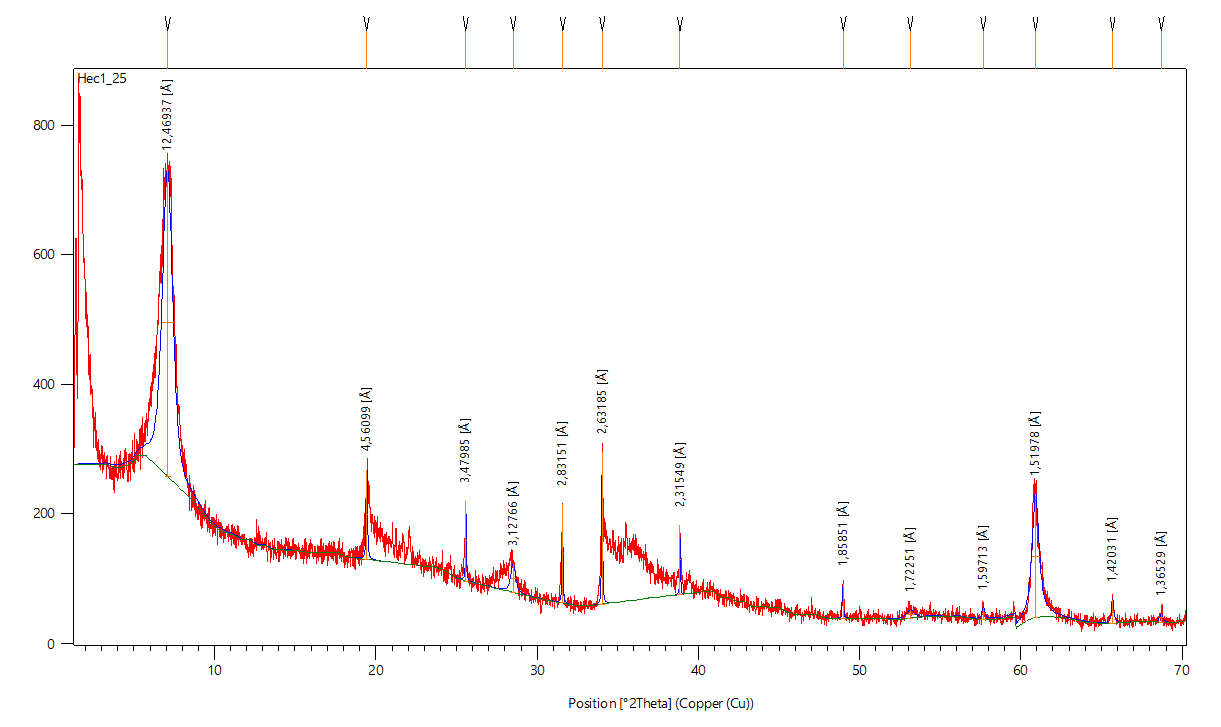
\includegraphics[scale=0.5]{Hec1.png}
  \caption{Zeigt das Pulverdiffraktogramm des Hectorits, dabei sind die Reflexe mit den Abstand der $d_{00n}$ Serie markiert.}
  \label{Hec1}
\end{figure}
\noindent
Aus Abbildung \ref{Hec1} ist ersichtlich, dass der $d_{001}$-Reflex bei einem Abstand von 12.46937 \AA liegt. 
Auf Grundlage dieses Werts lassen sich die theoretischen Abstände der $d_{00n}$-Serie berechnen. Dies erfolgt mithilfe der Formel \ref{d00n}.

\begin{equation}
  d_{00n}=\frac{d_{001}}{n}
  \label{d00n}
\end{equation}
\noindent
Die daraus erhaltenen Werte werden mit den in Abbildung \ref{Hec1} dargestellten experimentellen Daten verglichen und in Tabelle \ref{VergleichHec1} zusammengefasst.
\newpage
\begin{table}[h!]
\caption{\textit{Vergleich der aus Gleichung \ref{d00n} berechneten theoretischen Werte mit den experimentell bestimmten Werten aus Abbildung \ref{Hec1}.}}
\begin{center}
\begin{tabular}{|>{\columncolor{lightgray}}p{4cm}|>{\centering\arraybackslash}p{4cm}|>{\centering\arraybackslash}p{4cm}|}
   \hline
   \rowcolor{gray}
   &Berrechnete Werte& experimentellen Werte \\
   \hline
   $d_{001}$ [\AA]&12.46937& 12.46937\\
   \hline
   $d_{002}$ [\AA]&6.234685& Konnte nicht zugeordnet werden\\
   \hline
   $d_{003}$ [\AA]&4.156457& 4.56099\\
   \hline
   $d_{004}$ [\AA]&3.117343& 3.12766\\
   \hline
   $d_{005}$ [\AA]&2.493874& 2.63185\\
   \hline
  

\end{tabular}
\label{VergleichHec1}
\end{center}
\end{table}
\noindent
Aus den experimentellen Werten in Tabelle \ref{d00n} wird der Mittelwert gemäß Formel \ref{Mittelwert} berechnet.
\begin{equation}
  \overline{d}=\frac{\sum_{i}^{n}d_{00i}\cdot i}{n}=12.956
  \label{Mittelwert}
\end{equation}
\noindent
Zur Berechnung des Variationskoeffizienten CV werden die Gleichungen \ref{CV1} und \ref{CV2} herangezogen.
\begin{equation}
  \sqrt{\frac{\sum_{i}^{n}(d_{00i} \cdot i - \overline{d})^2}{n-1}} = 0.5787
  \label{CV1}
\end{equation}
\begin{equation}
  CV = \frac{100 \cdot 0.5797}{12.783} = 4.525 \%
  \label{CV2}
\end{equation}
\noindent
Somit beträgt die Schichtdicke des Hectorits \(12.955\,\text{\AA} \pm 4.535\,\%\). 
Die Synthese des Hectorits war zwar erfolgreich, jedoch treten im XRD auch Fremdreflexe auf. 
Diese stammen vermutlich von nicht vollständig umgesetztem \(\ce{ZnSiO4}\), was wahrscheinlich auf eine nicht vollständige umgesetztem der Fluoridsalze am 3. Tag schließen lässt.

\newpage
\subsection{Schichtdicke der Interkalationsverbindung}

Um die Schichtdicke der Interkalationsverbindung zu bestimmen, wird analog zu Abschnitt 3.1 vorgegangen. Das entsprechende XRD-Diffraktogramm ist in Abbildung \ref{Hec2} dargestellt. In Tabelle \ref{VergleichHec2} sind die berechneten Werte den experimentellen Ergebnissen gegenübergestellt.


\begin{figure}[!h]
  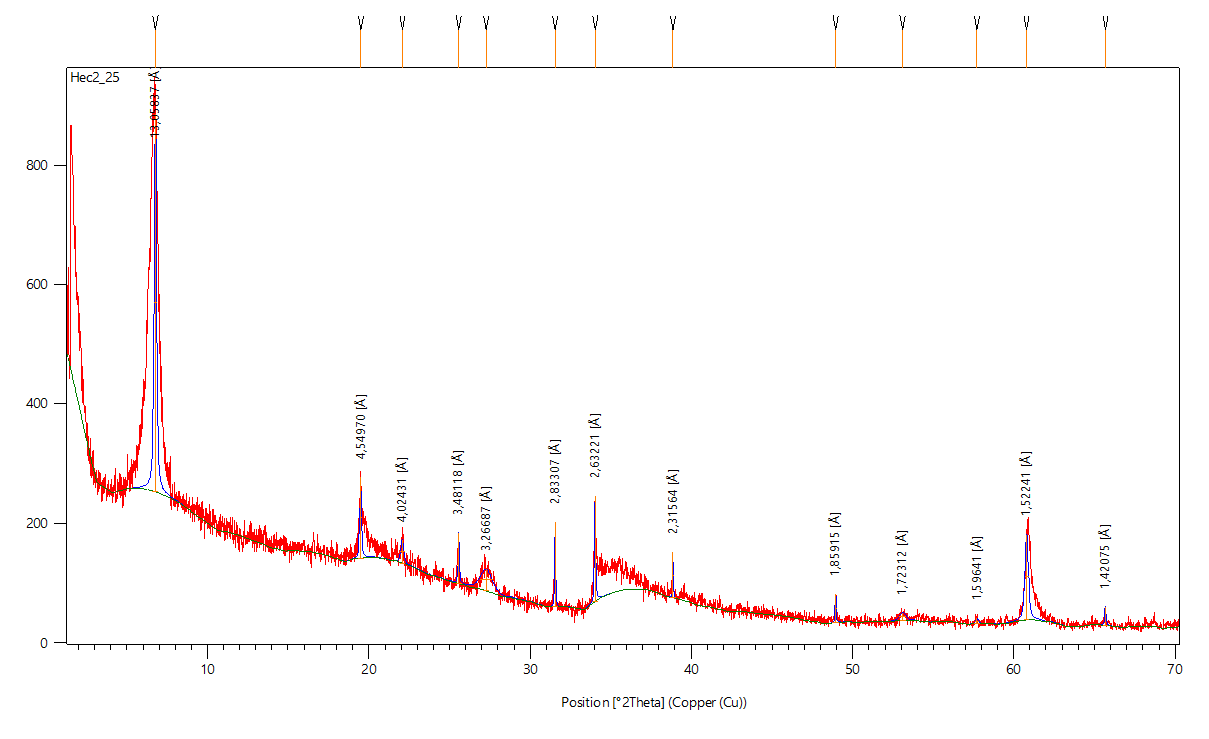
\includegraphics[scale=0.5]{Hec2.png}
  \caption{Zeigt das Pulverdiffraktogramm des Hectorits, dabei sind die Reflexe mit den Abstand der $d_{00n}$ Serie markiert.}
  \label{Hec2}
\end{figure}
\noindent
Der $d_{001}$-Reflex hat einen Abstand von 13.05837 \AA. Die Berrechneten Werte der Tabelle \ref{VergleichHec2} bezieht sich auf diesen Wert.
\begin{table}[h!]
\caption{\textit{Vergleich der aus Gleichung \ref{d00n} berechneten theoretischen Werte mit den experimentell bestimmten Werten aus Abbildung \ref{Hec2}.}}
\begin{center}
\begin{tabular}{|>{\columncolor{lightgray}}p{4cm}|>{\centering\arraybackslash}p{4cm}|>{\centering\arraybackslash}p{4cm}|}
   \hline
   \rowcolor{gray}
   &Berrechnete Werte& experimentellen Werte \\
   \hline
   $d_{001}$ [\AA]&13.05837& 13.058376\\
   \hline
   $d_{002}$ [\AA]&6.529185& Konnte nicht zugeordnet werden\\
   \hline
   $d_{003}$ [\AA]&4.352790& 4.54970\\
   \hline
   $d_{004}$ [\AA]&3.264583& 3.26687\\
   \hline
   $d_{005}$ [\AA]&2.611674& 2.63221\\
   \hline
  

\end{tabular}
\label{VergleichHec2}
\end{center}
\end{table}
\noindent
Aus Tabelle \ref{VergleichHec2} sowie den Gleichungen \ref{CV1} und \ref{CV2} ergibt sich, dass die Interkalationsverbindung einen mittleren Schichtabstand von
13.234 \AA \,mit einer Standardabweichung von 0.281 aufweist. Die relative Abweichung beträgt somit lediglich 2.12 \%. Daraus lässt sich schließen, dass die Einlagerung von \ce{[Cu(en)3]SO4} eine Vergrößerung der Schichtdicke zur Folge hat. Diese Vergrößerung beträgt etwa 0.279 \AA.
Dies weist auf eine unvollständige Einlagerung hin, da bei einer vollständigen Einlagerung ein größerer Schichtabstand zu erwarten wäre. Wenn das Kupfer nur in jede n-te Schicht eingelagert wird, resultiert daraus ein gemittelter Abstand. Infolgedessen ist nur ein n-tel der eigentlichen Schichtvergrößerung messbar.




\newpage









\newpage
\section{Zusammenfassung}
In diesem Versuch wurde erfolgreich die Verbindung \ce{Na_{0.5} \cdot nH2O [Zn_{2.5}Li_{0.5}](Si4O10)F2} synthetisiert. Zudem konnte die Einlagerung von \ce{[Cu(en)3]SO4} erfolgreich durchgeführt werden.
In der XRD-Messung wurden jedoch Verunreinigungen festgestellt. Diese stammen vermutlich von \ce{ZnSiO4}, 
das infolge einer unvollständigen Umsetzung mit den Fluoridsalzen in der Probe zurückgeblieben 
ist.



\noindent
Aus den XRD-Messungen lässt sich die Schichtdicke des Hectorits bzw. der Interkalationsverbindung berechnen. Für die Verbindung \ce{Na_{0.5} \cdot nH2O [Zn_{2.5}Li_{0.5}](Si4O10)F2}
ergibt sich eine Schichtdicke von
\mbox{$ 12.955\,\text{\AA} \pm 4.54\,\%$.}
Für die Interkalationsverbindung mit \ce{[Cu(en)3]SO4} ergab sich ein Wert von 
\mbox{$ 13.234\,\text{\AA} \pm 2.12\,\%$.}

\noindent
Somit ändert sich die Schichtdicke des Hectorits um  0.279 \AA, dies entspricht ca 2\% der Dicke. 
Das weißt auf eine nicht vollständige Einlagerung der kupferionen hin.



\newpage
\section{Literaturverzeichnis}
\printbibliography



\end{document}